\documentclass[11pt,a4paper]{article}

\usepackage[utf8]{inputenc}
\usepackage[MeX]{polski}
\usepackage{graphicx}
\usepackage{wrapfig}
\usepackage{color}
\usepackage{amsmath}
\usepackage{amssymb}
\usepackage[inkscapelatex=false]{svg}
\usepackage{array, makecell}
\usepackage{mhchem}
\usepackage{tabularx}
\usepackage{braket}
\usepackage{pdfpages}

\usepackage{multicol}
\usepackage{colortbl}
\usepackage[Export]{adjustbox}
\adjustboxset{max size={0.9\linewidth}{0.9\paperheight}}
\usepackage[colorlinks=true,linkcolor=red,citecolor=green]{hyperref}

\textwidth=16cm
\textheight=23cm
\topmargin=-2cm
\oddsidemargin=0cm

\setlength{\parindent}{0em}
\setlength{\parskip}{0.6em}
\setlength{\jot}{12pt}

\renewcommand{\arraystretch}{1.4}
\renewcommand\theadfont{\bfseries}

\newcommand{\todo}[1]{\textcolor{red}{TODO: #1}}

\begin{document}

\title{Ising model on random graphs with non-limited range of interactions}
\author{Dawid Karpiński,\\Supervisor: dr inż. Krzysztof Suchecki}
\date{}
\maketitle

\section*{Abstract}

The Ising model, renowned for its simplicity and effectiveness in capturing phase transitions, serves as a powerful tool to analyze the emergent properties of complex systems. The core objective of this research is to unravel the implications of non-limited interaction ranges in the context of random graphs. Traditional Ising models often assume a fixed range of interactions among neighboring spins. This work challenges that assumption by considering scenarios where interactions extend beyond the nearest neighbors, incorporating a broader and more realistic perspective on the interplay between spins.

\section{Introduction}
\begin{itemize}
\item brief historical overview of the Ising model and its significance in statistical physics
\item define the Ising model and its conventional assumptions
\item introduce the concept of random graphs and their relevance
\end{itemize}

\section{Literature Review}
\begin{itemize}
\item review existing literature on the Ising model
\item state the objectives and research questions.
\end{itemize}

\section{Theoretical Framework and Methodology}
\begin{itemize}
\item derive relevant equations and describe the mathematical foundations.
\end{itemize}

\section{Simulation Results and Analysis}

\todo{differences between J generation methods with k constant}

\begin{figure}[ht!]
    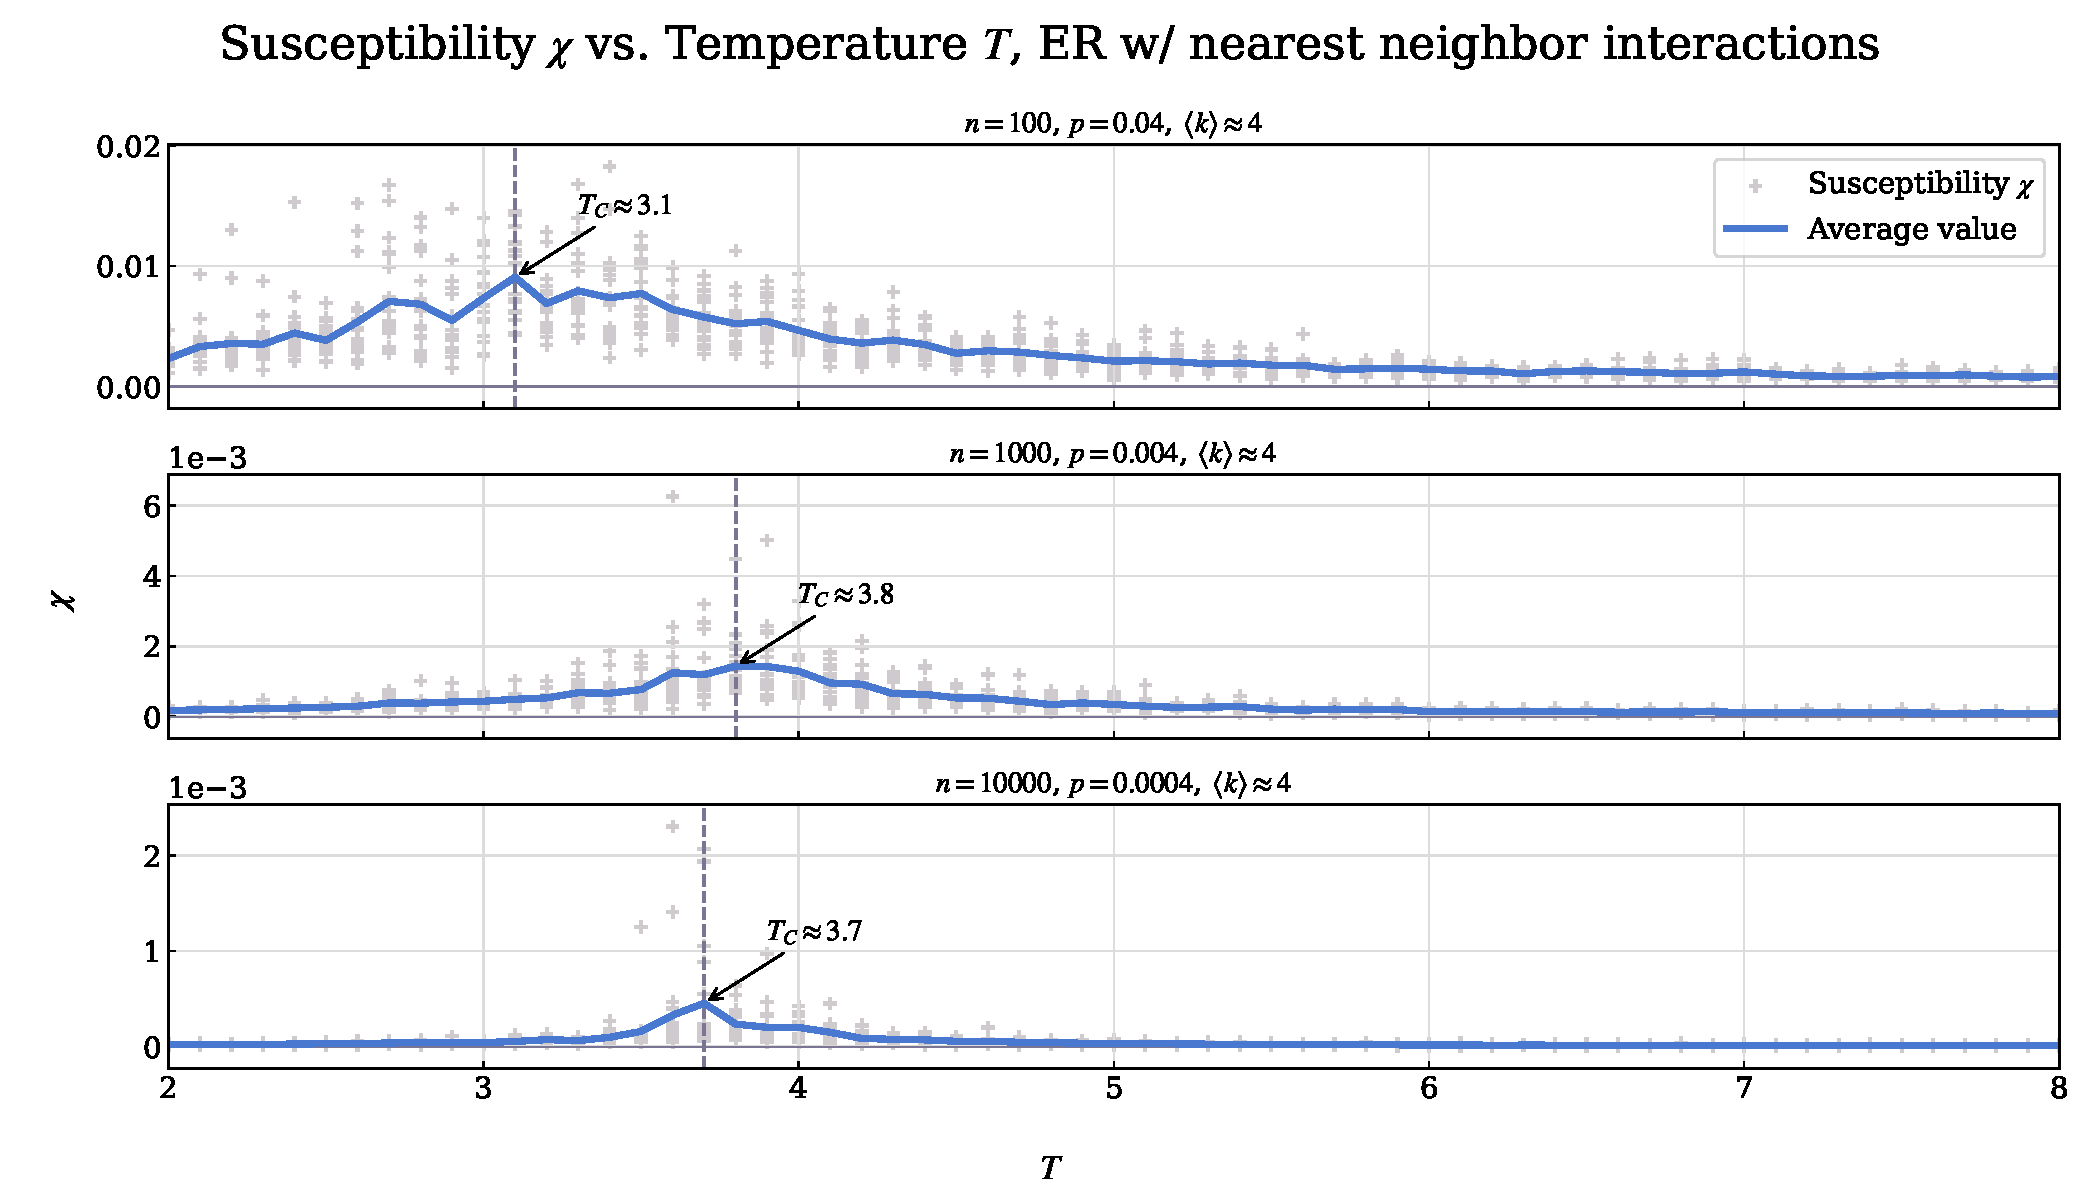
\includegraphics[width=\textwidth]{../figures/suscept_ER_nearest.pdf}
\end{figure}

\begin{figure}[ht!]
    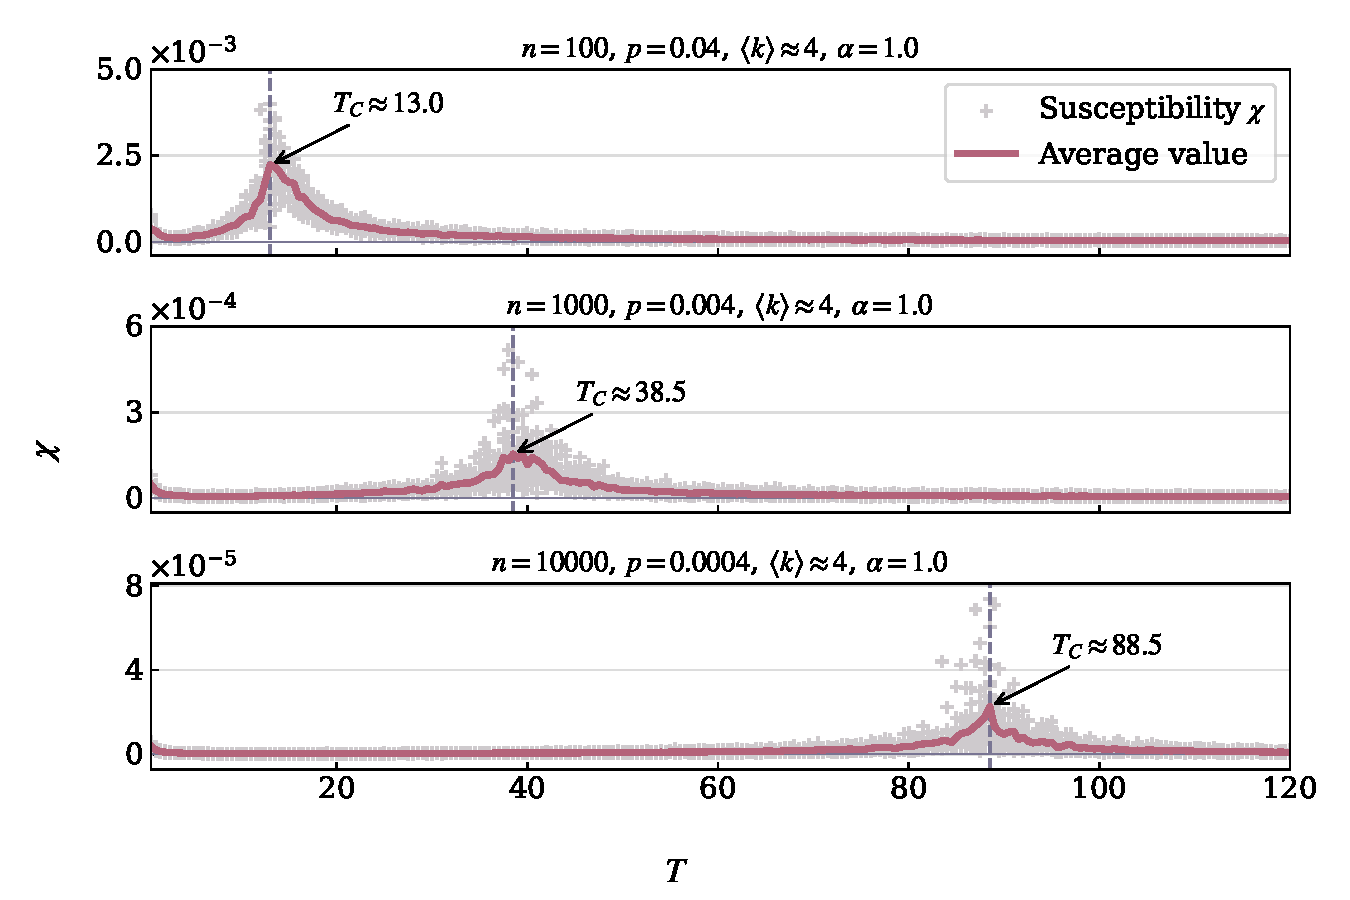
\includegraphics[width=\textwidth]{../figures/suscept_ER_single.pdf}
\end{figure}

\begin{figure}[ht!]
    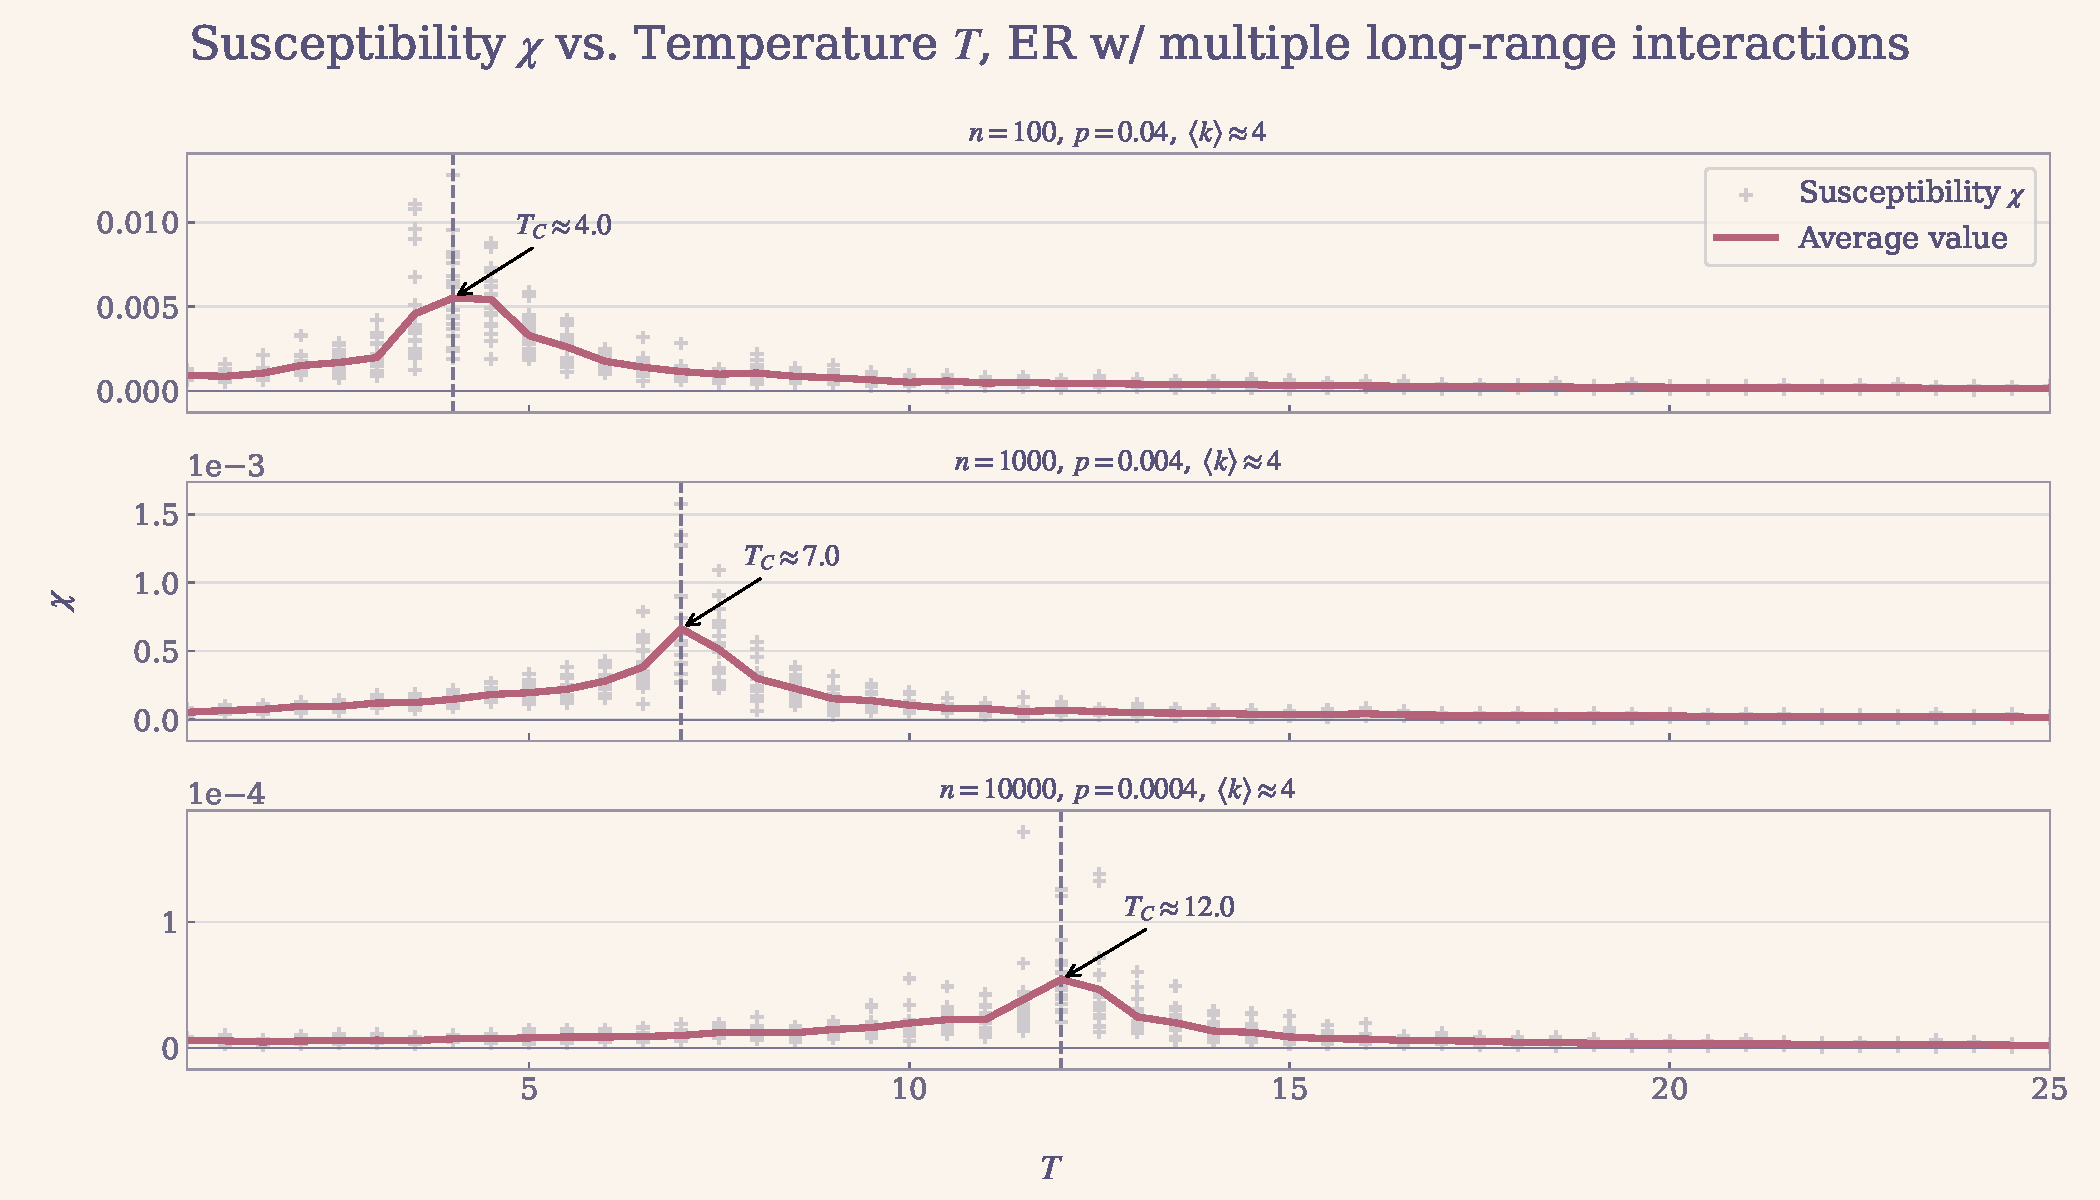
\includegraphics[width=\textwidth]{../figures/suscept_ER_multiple.pdf}
\end{figure}

\todo{e^{-\alpha k} vs 1/k^\alpha}

\todo{T_C vs. k with n kept constant}



\end{document}
